\section{Evaluation and Results}
\label{sec:evaluation-and-results}

We seek to evaluate whether \textsc{Appjudicator} is able to successfully
achieve its goal of distinguishing user-initiated network flows using UI
context, and whether it can do so with acceptable overhead. To determine whether
the app accomplishes its goal we perform a practical analysis and to measure the
app's resource cost we perform a performance evaluation. We now explain the
procedures used for each of these experiments and their results.

\subsection{Differentiating User-generated Flows}
\label{sec:differentiating-user-generated-flows}

The goal of this experiment is to determine whether \textsc{Appjudicator} can
successfully distinguish between network flows that were specifically initiated
by a human user and flows generated automatically by an app or the Android
system.

\subsubsection{Experimental Setup}
\label{sec:experimental-setup}

For this experiment, we tested the app both in an emulator an on a physical
Android device. The emulator test was performed on a virtual Google Pixel 4,
with API level 30 (the newest available). Physical tests were performed on a
real Google Pixel 3 phone running Android 11 with API level 30.

In both cases we used Google's UI Automator framework~\cite{uiautomator2020} to
automate the testing process. This tool is designed for automating UI tests as
part of an app development cycle, and provides features that make it ideal for
our experiments. The UI Automator can simulate various kinds of UI interactions,
including clicks, swipes, pressing hardware buttons, and even changing the
device's orientation. It can also perform actions in multiple apps in a single
run.

We use UI Automator to simulate a series of real life use cases that would lead
to a network request being made while \textsc{Appjudicator}'s accessibility
service is enabled. Then we simply check service's logs to see which flows it
marked as likely user-initiated. We run the test $x$ times to make sure the
results are reproducible, and not merely a coincidence of timing.

\subsubsection{Results}
\label{sec:practical-results}

% Use UI Automator to simulate real clicks, also find other apps that make
% background requests automatically
% Log whether each flow was user-generated, default-allowed, or automated
% What percentage of those flows were classified successfully?

\subsection{Performance Evaluation}
\label{sec:performance-evaluation}

To fulfill its purpose as an always-enabled enterprise network security tool,
\textsc{Appjudicator} has to be as unobtrusive to end users as possible. This is
especially important because the app performs some actions on every network
flow, so any latency added by it would be especially noticeable.

\subsubsection{Measuring Added Latency}
\label{sec:measuring-added-latency}

To measure the effect of \textsc{Appjudicator} on network communication speed,
we measure the total additional latency added by the app. We measure added
latency in all incoming and outgoing packets, but focus on the first packet of
new TCP connections in particular, because these require the most processing
time.

For this test, we run the app in an Android virtual machine simulating a Google
Pixel 4, on API level 30. We use POX's \texttt{forwarding.hub} module as an
OpenFlow controller. In this mode, the controller responds to every query with
an instruction to forward the flow to its destination~\cite{mccauley2015}. Local
network latency is not a part of this test, so the controller server runs on the
same physical host as the Android virtual machine. The two components still
communicate over a regular TCP connection. The SDN agent starts with an empty
table of flow rules, so it must send a \texttt{packet\_in} to the controller for
every new flow. \textsc{Appjudicator} caches responses from the controller as
new rules, so subsequent connections to the same IP address and port over the
same protocol will not trigger a \texttt{packet\_in}.
Section~\ref{sec:openflow-protocol} describes the OpenFlow protocol in more
detail.

We focus particularly on the added latency of the first packet in a TCP
connection because this is where the system does the most processing. The start
of a new flow requires an SDN flow table lookup and possibly communication with
the SDN controller. Creating a new TCP connection requires allocating more
memory than a new UDP connection because metadata such as the current connection
state and most recent sequence number need to be stored in a lookup table.
Subsequent packets in a TCP flow, and all packets in UDP flows require less
processing overhead.

We configure the app to log a timestamp when a packet is first intercepted by
the VPN. \textsc{Appjudicator}'s VPN service parses the packet and determines
whether it is part of an existing connection or not, and adds it to a queue. If
it is the start of a new connection, the VPN service queries the SDN agent and
continues processing other packets while waiting for a response. The SDN agent
performs a flow table lookup, and sends a \texttt{packet\_in} to the SDN
controller if it fails to find a matching rule. If this is the case it waits for
a response from the controller, then performs a flow mod operation to cache the
result as a new rule. Finally the SDN agent instructs the VPN service to drop or
forward the flow. In this test all flows are allowed, so the VPN service removes
the packet from its queue and writes it to the correct network interface file
descriptor.\footnote{Figure~\ref{fig:packet-flow-chart} illustrates this
process.} Now that all of \textsc{Appjudicator}'s processing is finished a
second timestamp is logged. The earlier timestamp is the time the packet would
have been sent to the network without our system's interference, and the second
timestamp is the time it actually was sent. The difference is the total latency
added by the app.

In this test the app is configured to write the recorded time differences for
all packets to a file. Time differences for TCP SYN packets are also logged to
another file. Timestamps are created using Android's
\texttt{SystemClock.elapsedRealtimeNanos()} method, which gets the number of
nanoseconds since the system was booted.~\cite{androidsystemclock}

\subsubsection{Latency Test Results}
\label{sec:latency-test-results}

There were 1104 packet timing traces logged during the sampling period, of which
two were removed as outliers, leaving 1102 data points. The average added
latency among all packets was 5.14 milliseconds, with a standard deviation of
3.44 milliseconds.

During the sampling period 184 TCP SYN timing traces were logged, of which five
were removed as outliers, leaving 179 data points. These packets had 
higher added latency than others, and their added latency varied more. The
average added latency among TCP SYN packets was 14.64 milliseconds, with a
standard deviation of 16.77 milliseconds.

In our sample, 95\% of packets were processed with less than 10 milliseconds
of total added delay. On a 60 Hz display one frame lasts 16 milliseconds, so any
delay less than this is imperceptible to users.
Figure~\ref{fig:added-delay-chart} charts the full results of this test.

\begin{figure}[h]
    \centering
	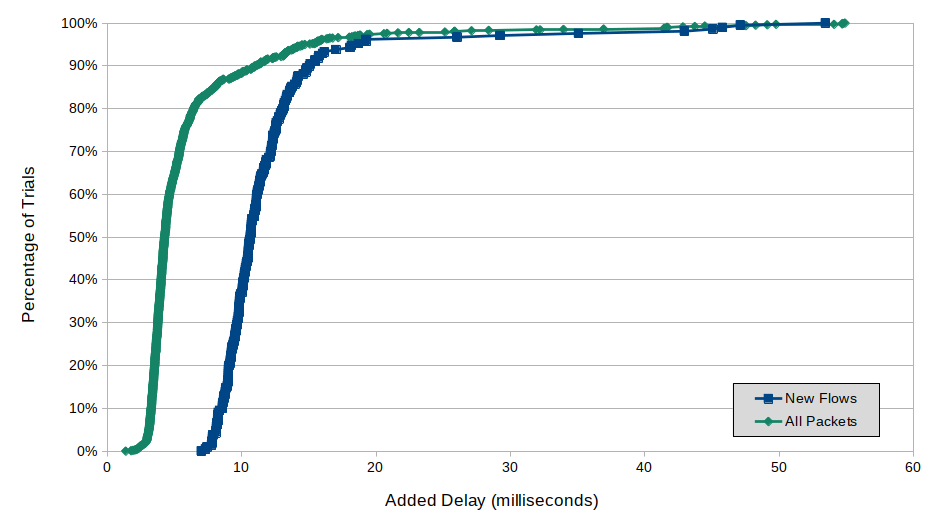
\includegraphics[width=\textwidth]{added-delay.png}
	\caption{Total latency added by \textsc{Appjudicator}}
	\label{fig:added-delay-chart}
\end{figure}

\subsubsection{Measuring Resource Overhead}
\label{sec:measuring-resource-overhead}

\textsc{Appjudicator} has costs in both added latency and increased resource
consumption. Running the VPN service, accessibility service, and SDN agent in
the background consumes additional processing cycles, memory, and battery life.
We measure the resource overhead with Android Studio's
Profiler.~\cite{androidprofiler}

This test was performed on an Android virtual machine simulating a Google Pixel
4, on API level 30. We ran the app the accessibility service, VPN service, and
SDN agent all enabled while recording its CPU, memory, and energy usage with
Android Studio's Profiler. The test lasted for 30 minutes, during which time we
used various other apps including Chrome, Termux, and F-Droid while
\textsc{Appjudicator} ran in the background.

During the trial, \textsc{Appjudicator}'s memory usage remained relatively
constant. It peaked at at 150.1 MB, with an average of 137.8 MB. Its processor
usage also usually remained low, averaging 5\% of the virtual machine's CPU but
occasionally spiking as high as 39\%. The profiler categorized the app's energy
usage as ``light,'' because it used only minor CPU resources and did not use any
location resources, wake locks, or alarms.

Based on these results, we conclude that \textsc{Appjudicator} has a minor
impact on CPU, memory, and battery usage on modern hardware, and therefore could
be used effectively as an always-on background security application.

\newpage

